%% LyX 2.0.4 created this file.  For more info, see http://www.lyx.org/.
%% Do not edit unless you really know what you are doing.
\documentclass[ngerman]{beamer}
\usepackage[T1]{fontenc}
\usepackage[latin9]{inputenc}
\usepackage{listings}
% footnotesize
\lstset{ %
language=Python,                % choose the language of the code
basicstyle=\scriptsize,       % the size of the fonts that are used for the code
numbers=left,                   % where to put the line-numbers
numberstyle=\scriptsize,      % the size of the fonts that are used for the line-numbers
stepnumber=1,                   % the step between two line-numbers. If it is 1 each line will be numbered
numbersep=5pt,                  % how far the line-numbers are from the code
backgroundcolor=\color{white},  % choose the background color. You must add \usepackage{color}
showspaces=false,               % show spaces adding particular underscores
showstringspaces=false,         % underline spaces within strings
showtabs=false,                 % show tabs within strings adding particular underscores
frame=single,           % adds a frame around the code
tabsize=2,          % sets default tabsize to 2 spaces
captionpos=b,           % sets the caption-position to bottom
breaklines=true,        % sets automatic line breaking
breakatwhitespace=false,    % sets if automatic breaks should only happen at whitespace
escapeinside=\`\`,
%escapeinside={\%*}{*)}          % if you want to add a comment within your code
}

\newcommand\red[1]{{\color{red}#1}}

\newcommand\redit[1]{{\color{red}\textit{#1}}}

\setcounter{secnumdepth}{3}
\setcounter{tocdepth}{3}
\usepackage{babel}
\usepackage{graphicx}
\ifx\hypersetup\undefined
  \AtBeginDocument{%
    \hypersetup{unicode=true}
  }
\else
  \hypersetup{unicode=true}
\fi
\usepackage{breakurl}

\makeatletter
%%%%%%%%%%%%%%%%%%%%%%%%%%%%%% Textclass specific LaTeX commands.
 % this default might be overridden by plain title style
 \newcommand\makebeamertitle{\frame{\maketitle}}%
 \AtBeginDocument{
   \let\origtableofcontents=\tableofcontents
   \def\tableofcontents{\@ifnextchar[{\origtableofcontents}{\gobbletableofcontents}}
   \def\gobbletableofcontents#1{\origtableofcontents}
 }
 \long\def\lyxframe#1{\@lyxframe#1\@lyxframestop}%
 \def\@lyxframe{\@ifnextchar<{\@@lyxframe}{\@@lyxframe<*>}}%
 \def\@@lyxframe<#1>{\@ifnextchar[{\@@@lyxframe<#1>}{\@@@lyxframe<#1>[]}}
 \def\@@@lyxframe<#1>[{\@ifnextchar<{\@@@@@lyxframe<#1>[}{\@@@@lyxframe<#1>[<*>][}}
 \def\@@@@@lyxframe<#1>[#2]{\@ifnextchar[{\@@@@lyxframe<#1>[#2]}{\@@@@lyxframe<#1>[#2][]}}
 \long\def\@@@@lyxframe<#1>[#2][#3]#4\@lyxframestop#5\lyxframeend{%
   \frame<#1>[#2][#3]{\frametitle{#4}#5}}
 \def\lyxframeend{} % In case there is a superfluous frame end
 \long\def\lyxplainframe#1{\@lyxplainframe#1\@lyxframestop}%
 \def\@lyxplainframe{\@ifnextchar<{\@@lyxplainframe}{\@@lyxplainframe<*>}}%
 \long\def\@@lyxplainframe<#1>#2\@lyxframestop#3\lyxframeend{%
   \frame<#1>[plain]{\frametitle{#2}#3}}

\makeatother

\begin{document}

\title{Informationsextraktion aus Websites}


\author{Michael Haas <haas@computerlinguist.org>}


\institute{Service-Center Forschungsdaten, Universit�t Mannheim}


\date{22.01.2013}

\makebeamertitle

\lyxframeend{}\lyxframe{Lessons Learned - Kontext}
\begin{itemize}
\item Mein Hintergrund: B.A. Computerlinguistik, Universit�t Heidelberg
\item Projekte am Service-Center:

\begin{itemize}
\item Manuel Trenz: Beobachtung der Preisver�nderungen einer gegebenen Menge
an Produkten auf Online-Shops und Preisvergleichern
\item Dominic Nyhuis: Durchsuchen der Online-Archive von 10 Zeitungen per
Screen Scraping
\item Georg Wernicke: NER und Sentiment-Analyse auf Zeitungsartikeln
\end{itemize}
\item Ziele f�r heute

\begin{itemize}
\item Tutorial Screen Scraping
\item Folien als Referenz
\item Lessons Learned als Hinweise/best practices
\end{itemize}
\end{itemize}

\lyxframeend{}


\lyxframeend{}\lyxframe{Aufgabe}
\begin{itemize}
\item Kunde ben�tigt Daten von Website
\item Manuelle Extraktion mit HiWis und Copy\&Paste zu aufwendig
\item Automatisieren!
\end{itemize}

\lyxframeend{}

\begin{frame}[fragile]\frametitle{Python}

Konkret: Kunde m�chte Produktpreise �ber l�ngeren Zeitraum �berwachen

\begin{lstlisting}
>> import urllib2
>> content = urllib2.urlopen("http://host/produkt/id")
HTTPError: `\red{HTTP Error 403: denied}` - contact webmaster@host
\end{lstlisting}
\end{frame}

\begin{frame}[fragile]\frametitle{Python - Ninja Level 1}

Website mag unseren User-Agent nicht!

\begin{lstlisting}
>> request = urllib2.Request("http://host/produkt/123")
>> request.add_header('User-Agent', 'Mozilla/5.0')
>> opener = urllib2.build_opener() 
>> content = opener.open(request).read() 
>> content[0:30]
'<!DOCTYPE HTML><html lang="de"' 
\end{lstlisting}
\end{frame}

\begin{frame}[fragile]\frametitle{Python - Iteration}

Kunde will mehrere Produkte �berwachen

\begin{lstlisting}
>> for p in products*100: 
    request = urllib2.Request("http://host/produkt/" + p) 
    request.add_header('User-Agent', 'Mozilla/5.0') 
    opener = urllib2.build_opener()
    content = opener.open(request).read() 
HTTPError: `\red{HTTP Error 421: too fast}` - contact webmaster@host
\end{lstlisting}
\end{frame}

\begin{frame}[fragile]\frametitle{Python - Ninja Level 2}

\begin{lstlisting}
>> import time
>> for p in products*100:
    request = urllib2.Request("http://host/product/" + p)
    request.add_header('User-Agent', 'Mozilla/5.0') 
    opener = urllib2.build_opener() 
    content = opener.open(request).read() 
    time.sleep(5)
\end{lstlisting}
\end{frame}

\begin{frame}[fragile]\frametitle{Python - Paranoid Ninja}

Admin k�nnte Access Logs �berwachen - Abst�nde der Zugriffe zuf�llig
halten!

\begin{lstlisting}
>> import random,time
>> for p in products*100:
    request = urllib2.Request("http://host/product/" + p)
    request.add_header('User-Agent', 'Mozilla/5.0')
    opener = urllib2.build_opener() 
    content = opener.open(request).read() 
    time.sleep(random.uniform(1,5))
\end{lstlisting}
\end{frame}

\begin{frame}[fragile]\frametitle{Python - there is a lib for that}

Alles zu kompliziert! Besser:

\begin{lstlisting}
$ sudo easy_install-2.7 leechi
$ ipython2
>> import leechi
>> l = leechi.Leechi()
>> for p in product:
    content = l.fetchDelayed("http://host/product/" + p)
\end{lstlisting}
\end{frame}

\begin{frame}[fragile]\frametitle{Python - Leechi}

\begin{lstlisting}
>> l = leechi.Leechi(cookies=True, retry=3)
>> l.chooseRandomUA()
>> l.setCustomUA("Wget/1.9.1")
>> handle = l.obtainHandle("http://host/")
>> content = handle.read()
>> handle = l.obtainHandleDelayed("http://host/")
\end{lstlisting}
\end{frame}

\begin{frame}[fragile]\frametitle{Python - Leechi - Source}
\begin{itemize}
\item \href{http://github.com/mhaas/leechi/}{http://github.com/mhaas/leechi/}
\item \href{http://pypi.python.org/pypi/Leechi/0.2}{http://pypi.python.org/pypi/Leechi/0.2}
\item Send Patches:

\begin{itemize}
\item Periodisches Wechseln von UA
\item Unterst�tzung (anonymer) Proxy-Server
\item Tests
\end{itemize}
\end{itemize}
\end{frame}


\begin{frame}[fragile]\frametitle{Python - HTML Parsing}
Und nun?

\begin{lstlisting}
>> content = """<html><body>
                <p class="price">preis ist: 5euro</p>
                </body></html>"""
>> import re
>> re.search(ur'preis ist: (\d{0,4})euro', content).group(1) 
'5'
\end{lstlisting}
\end{frame}

\begin{frame}[fragile] \frametitle{Python - HTML Parsing - Nie RegEx}
\begin{itemize}
\item HTML/XML sind kontextfreie Sprachen
\item Regul�re Ausdr�cke beschreiben regul�re Sprachen
\item Kontextfreie Sprachen sind m�chtiger als regul�re Sprachen%
\footnote{``Parsing HTML with regex summons tainted souls into the realm of
the living.''\href{http://stackoverflow.com/a/1732454}{http://stackoverflow.com/a/1732454}%
}
\end{itemize}
\end{frame}

\begin{frame}[fragile]\frametitle{Python - HTML Parsing - BeautifulSoup}
\begin{itemize}
\item Besser: BeautifulSoup 4
\item Kann alles, auch Tagsuppe:

\begin{itemize}
\item fehlende schlie�ende Tags
\item mangelhaft kodierte Sonderzeichen
\end{itemize}
\item \href{http://www.crummy.com/software/BeautifulSoup/}{http://www.crummy.com/software/BeautifulSoup/}
\end{itemize}
\end{frame}

\begin{frame}[fragile]\frametitle{Python - HTML Parsing - BeautifulSoup - Navigation}

HTML-Attribut \textit{class} sehr n�tzlich als Ziel.

\begin{lstlisting}
$ sudo easy_install-2.7 beautifulsoup4
$ python2
>> content = """<html>
                 <body>
                  <p `\redit{class=''price''}`>preis ist: 5e</p>
                 </body>
                </html>"""
>> from bs4 import BeautifulSoup
>> soup = BeautifulSoup(content)
>> soup.find(`\red{class\_=''price''}`)
<p class="price">preis ist: 5e</p> 
\end{lstlisting}
\end{frame}

\begin{frame}[fragile]\frametitle{Python - HTML Parsing - BeautifulSoup - Navigation}

Container f�r Listen

\begin{lstlisting}
>> content = """<ul `\redit{id=''priceList''}`>
                <li>preis: 5e</li>
                <li>preis: 10e</li>
                <li>preis: 15e</li>
                </ul>"""
>> priceList = soup.find('ul', `\red{id='priceList'}`)
>> for node in priceList.children: # priceList.contents
    re.search(ur"preis: (\d{1,4})e", node.string).group(1)
5 
10 
15
\end{lstlisting}
\end{frame}

\begin{frame}[fragile]\frametitle{Python - HTML Parsing - BeautifulSoup - Navigation}

Durch den Baum hangeln

\begin{lstlisting}
>> content = """<div>
                 <h1 `\redit{class=''section-header''}`>Preise</h1>
                 <h3>Zubehoer</h3>
                 <ul>
                  <li>preis: 5e</li>
                 </ul>
                </div>"""
>> soup.div.h1.nextSibling.nextSibling
<ul><li>preis: 5e</li></ul> 
>> soup.div.contents[2] 
<ul><li>preis: 5e</li></ul> 
>> soup.find(`\red{class\_=''section-header''}`).nextSibling.nextSibling
<ul><li>preis: 5e</li></ul> 
\end{lstlisting}
\end{frame}

\begin{frame}[fragile]\frametitle{Python - HTML Parsing - BeautifulSoup - Navigation}

\begin{lstlisting}
>> for string in soup.strings:
    print string
Preise
Zubehoer
preis: 5e 
\end{lstlisting}

\begin{itemize}
\item \textit{soup.stripped\_strings}: ohne Leerzeichen
\item \textit{soup.descendants}: depth-first search
\end{itemize}
\end{frame}


\lyxframeend{}\lyxframe{BeautifulSoup - Suchen}
\begin{itemize}
\item Nach Tag-Namen
\item Nach Attributen
\item Nach Text
\item Kombinationen
\end{itemize}

\lyxframeend{}

\begin{frame}[fragile]\frametitle{Python - HTML Parsing - BeautifulSoup - Suchen - Tag}

\begin{lstlisting}
>> soup.h1
<h1 class="section-header">Preise</h1>
>> soup.find('h1') 
<h1 class="section-header">Preise</h1> 
>> soup.find_all('h1')[0]
<h1 class="section-header">Preise</h1> 
\end{lstlisting}
\end{frame}

\begin{frame}[fragile]\frametitle{Python - HTML Parsing - BeautifulSoup - Suchen - Attribut}

\begin{lstlisting}
>> content = """<div>
                 <h1>Preise</h1>
                 <h3 `\redit{id=''header''}`>Zubehoer</h3>
                 <ul>
                  <li>preis: 5e</li>
                 </ul>
                </div>'
>> soup.find(id="header")
<h3 id="header">Zubehoer</h3>
>> soup.find("h3", id="header")
<h3 id="header">Zubehoer</h3>
>> soup.find(id=re.compile('head'))
<h3 id="header">Zubehoer</h3> 
>> soup.find(id=re.compile('head'))["id"]
'header' 
\end{lstlisting}
\end{frame}

\begin{frame}[fragile]\frametitle{Python - HTML Parsing - BeautifulSoup - Suchen - Text}

\begin{lstlisting}
>> soup.find(text="Zubehoer")
u'Zubehoer'
>> soup.find(text="Zubehoer").parent 
<h3 id="header">Zubehoer</h3>
>> soup.find_all(text=True)
[u'Preise', u'Zubehoer', u'preis: 5e'] 
>> soup.find_all(text=re.compile("[pP]reis"))
[u'Preise', u'preis: 5e'] 
\end{lstlisting}
\end{frame}


\lyxframeend{}\lyxframe{Zwischenstand}

Wir k�nnen:
\begin{itemize}
\item unerkannt Content herunterladen
\item Content parsen und Information extrahieren
\end{itemize}
Spezialfall: Suchanfragen auf Websites automatisieren!


\lyxframeend{}

\begin{frame}[fragile]\frametitle{Suchmasken - Automatisierung von Formularen}
\begin{itemize}
\item Suchmasken sind \emph{\textless form\textgreater}-Objekte mit \emph{\textless input\textgreater}-Feldern
\item �bermittlung per HTTP GET oder POST
\item Achtung: ben�tigt oft Cookies f�r Session Management! 
\begin{lstlisting}
Leechi(cookies=True)
\end{lstlisting}

\end{itemize}
\end{frame}

\begin{frame}[fragile]\frametitle{Suchmasken - Automatisierung von Formularen}

\href{http://de.wikipedia.org/wiki/Spezial:Suche}{http://de.wikipedia.org/wiki/Spezial:Suche}

\begin{lstlisting}[language=HTML]
<form id="search" `\red{method=''get''}` `\red{action=''/w/index.php''}`>
    <input value="Spezial:Suche" name="title" type="hidden" />
    <input value="default" name="profile" type="hidden" />
    <input id="searchText" `\red{name=''search''}`/> 
    <input value="Search" name="fulltext" type="hidden" /> 
    <input type="submit" value="Volltext" />
</form>
\end{lstlisting}
\end{frame}

\begin{frame}[fragile]\frametitle{Suchmasken - GET Request}

\href{http://de.wikipedia.org/w/index.php?title=Spezial\%3ASuche&profile=default&search=katze&fulltext=Search}{http://de.wikipedia.org/w/index.php?title=Spezial\%{}3ASuche\&{}profile=default\&{}search=Gepardenforelle\&{}fulltext=Search}

\begin{lstlisting}
>> import urllib
>> params = {   "title" : "Spezial:Suche",
                "fulltext" : "Search",
                "search" : "katze",
                "profile": "Default" }
>> urllib.urlencode(params)
'profile=Default&fulltext=Search&search=katze&title=Spezial%3ASuche'
>> content = l.fetchDelayed("http://de.wikipedia.org/w/index.php?" + urllib.urlencode(params))
\end{lstlisting}
\end{frame}

\begin{frame}[fragile]\frametitle{Suchmasken - POST Request}
\begin{itemize}
\item POST als Request Method
\item Parameter als separaten Wert �bergeben
\end{itemize}
\begin{lstlisting}
>> l.obtainHandleDelayed(baseURL, urllib.urlencode(params))
\end{lstlisting}
\end{frame}

\begin{frame}[fragile]\frametitle{Suchmasken - Wikipedia - Pagination}

Suchergebnisse �ber mehrere Seiten verteilt
\begin{itemize}
\item Zus�tzliche Parameter

\begin{itemize}
\item \emph{offset}
\item \emph{limit}
\end{itemize}
\end{itemize}
\begin{lstlisting}
>> params = {   offset : "20,
                limit : "20",
                "title" : "Spezial:Suche",
                "fulltext" : "Search",
                "search" : "katze",
                "profile": "Default" }
\end{lstlisting}


\href{http://de.wikipedia.org/w/index.php?title=Spezial:Suche&limit=20&offset=20&redirs=0&profile=default&search=katze}{http://de.wikipedia.org/w/index.php?title=Spezial:Suche\&{}limit=20\&{}offset=20\&{}redirs=0\&{}profile=default\&{}search=katze}

\end{frame}

\begin{frame}[fragile]\frametitle{Suchmasken - Wikipedia - Alle Links extrahieren}

Beispiel: extrahiere alle Links aus Suchergebnis

\begin{lstlisting}
>> while has_more_results():
    params["offset"] = offset
    content = l.fetchDelayed("http://..?" + urllib.urlencode(params))
    soup = BeautifulSoup(content)
    for node in soup.find_all("div", class\_="mw-search-result-heading"): 
        results.append(node.a["href"]) 
    offset += 20 
\end{lstlisting}
\end{frame}


\lyxframeend{}\lyxframe{Suchmasken - has\_more\_results()?}

Wann haben wir alle Ergebnisse gesehen?
\begin{itemize}
\item Server liefert auf letzter Seite weniger Ergebnisse als \emph{limit}
\item Server liefert Fehler 404, 500 bei zu gro�em \emph{limit}
\item Server liefert doppelte Ergebnisse bei zu gro�em \emph{limit}
\item Am Besten: Vergleich mit Anzahl Ergebnisse - nicht immer korrekt
\item \red{Keine} allgemeing�ltige Formel!
\end{itemize}

\lyxframeend{}


\lyxframeend{}\lyxframe{Zusammenfassung}
\begin{itemize}
\item Kommunikation mit Server �ber Leechi
\item Extraktion von Informationen aus DOM-Baum �ber BeautifulSoup
\item Suchmasken: GET/POST requests mit allen Parametern, Cookies!
\item Ende der Ergebnisliste: here be dragons!
\end{itemize}

\lyxframeend{}


\lyxframeend{}\lyxframe{Werkzeugkasten}
\begin{itemize}
\item Python, BeautifulSoup, Leechi
\item Browser: ``View Source'', DOM Inspector
\item Firefox: Web Console, Live HTTP Headers
\item Wireshark
\end{itemize}

\lyxframeend{}


\lyxframeend{}\lyxplainframe{Wireshark}

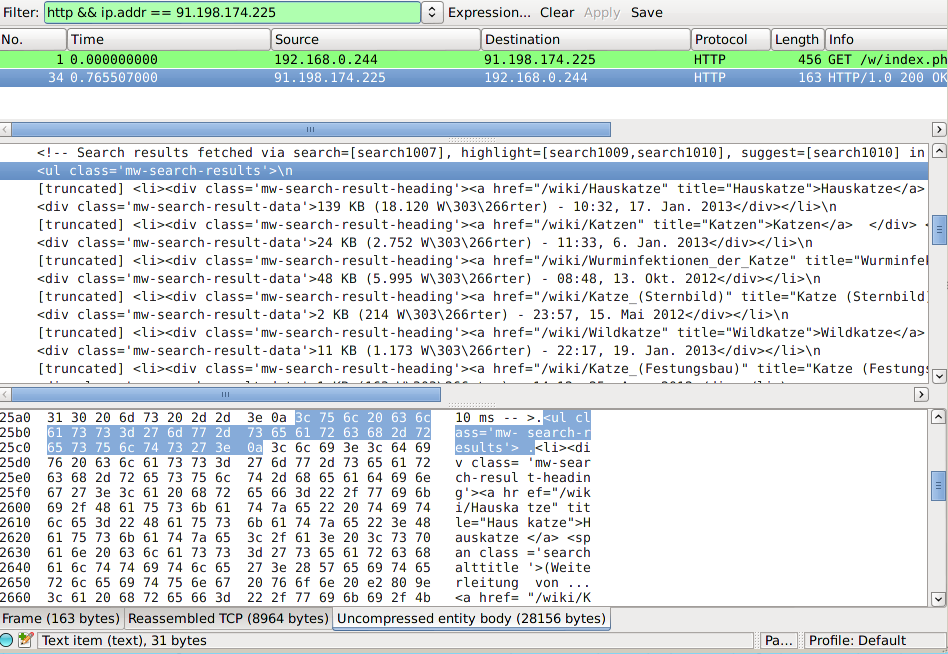
\includegraphics[width=0.9\paperwidth]{wireshark-wikipedia-katze}


\lyxframeend{}

\begin{frame}[fragile]\frametitle{Lessons Learned - Encodings}
\begin{itemize}
\item Encoding matters: Parameter passend kodieren
\item Encoding aus HTTP-Headern: \emph{charset}-Parameter in \emph{Content-Type}
\item Alternative: \emph{\textless meta http-equiv=\textquotedbl{}Content-Type\textquotedbl{} ...\textgreater}

\item Achtung: \textquotedbl{}\emph{latin-}1\textquotedbl{}\emph{ }bedeutet
oft \textquotedbl{}\emph{cp1252}\textquotedbl{}
\end{itemize}
\begin{lstlisting}
>> params = {"query" : u"M�ller"`\red{.decode(''utf-8'')}`}
>> l.fetchDelayed("http://host/", urllib.urlencode(params))
\end{lstlisting}
\end{frame}

\begin{frame}[fragile]\frametitle{Lessons Learned - Tests}
\begin{itemize}
\item Umfangreichere Projekte: Unit-Test-Frameworks!
\end{itemize}
\begin{lstlisting}
>> items = crawl("Katze", from="01.01.", to="01.03.")
>> assert(len(items) == 84)
\end{lstlisting}

\begin{itemize}
\item Alternative: ungl�cklicher Kunde, ungl�cklicher Entwickler
\end{itemize}
\end{frame}


\lyxframeend{}\lyxframe{Lessons Learned - Parsers}
\begin{itemize}
\item Nicht jeder Parser in BeautifulSoup4 kommt mit jeder Tagsuppe klar
\footnote{http://www.crummy.com/software/BeautifulSoup/bs4/doc/\#installing-a-parser%
}
\item Gut, aber langsam: \emph{html5lib - BeautifulSoup(content, ``html5lib'')}
\item Auch \emph{html5lib} funktioniert nicht immer; \emph{lxml} auch brauchbar
\item Parsing-Fehler \red{subtil} - DOM-Tree laden und wieder serialisieren
\item Tests schreiben!
\end{itemize}

\lyxframeend{}


\lyxframeend{}\lyxframe{Lessons Learned - Session Management}
\begin{itemize}
\item Session Management f�r einige Websites notwendig
\item Session Management per Cookie 
\item Oder: Per Parameter in GET-Request - muss dann extrahiert \& �bergeben
werden!
\item Selten: verpflichtende, wechselnde Parameter (form input) - muss bei jedem Seitenwechsel
extrahiert werden
\end{itemize}

\lyxframeend{}


\lyxframeend{}\lyxframe{Bonus: AJAX}
\begin{itemize}
\item Keine Daten im HTML-Source, aber im DOM-Baum
\item Dynamische Website mit AJAX
\item Content wird dynamisch nachgeladen als JSON oder XML und DOM-Baum
modifiziert
\item URL finden:

\begin{itemize}
\item Javascript-Code lesen
\item Wireshark
\item Browser-Extension
\end{itemize}
\end{itemize}

\lyxframeend{}

\begin{frame}[fragile]\frametitle{Bonus: AJAX}

\begin{lstlisting}
>> import json
>> content = urllib.urlopen('https://ajax.googleapis.com/ajax/services/feed/load?v=1.0&q=http://www.digg.com/rss/index.xml').read()
>> data = json.loads(content)
>> data["responseData"]["feed"]["author"] 
u'Digg'
\end{lstlisting}
\end{frame}


%%\lyxframeend{}\lyxframe{Resourcen}




%%\lyxframeend{}
\end{document}
